\documentclass{article}
\usepackage{listings}
\usepackage{graphicx}

\newcommand{\SolutionName}{ApiProtocols}
\newcommand{\ProjectName}{ApiProtocols}

\newcommand{\code}[1]{\lstinline{#1}}

\title{\ProjectName{} Example}
\date{}


\begin{document}
\maketitle
\begin{abstract}
This example shows how contracts allow you to make the often implicit API protocol on
a class explicit. API protocols are rules about what states an object
goes through and when it is okay to call particular methods and
properties. Clients are supposed to follow these rules, but often
clients have to discover these rules by trial-and-error.

The example consists of a library
exposing a class that has to be used in a certain way. A separate
client application makes use of this class.

In this sample, you will learn how to write contracts that describe
protocols on your classes and how such protocols are enforced on clients.
\end{abstract}

\newcommand\codefamily\sffamily
\lstset{language={[Sharp]C},mathescape=true,flexiblecolumns=true,morekeywords={Requires,Ensures,Invariant},basicstyle=\codefamily\small,literate={->}{{$\rightarrow$}}{2}{<<}{{$\langle$}}{2}{>>}{{$\rangle$}}{2}{!}{{\textbf{!}}}{2},frame=lines,moredelim=[is][\itshape]{@}{@},captionpos=b,numberstyle=\tiny,stepnumber=1,numbersep=2pt}

\section{Adding the Contract Library Reference}
If you are using Visual Studio 2008, or if you for 
some reason want to target a pre-v4 .NET runtime, then you need to:
\begin{itemize}
\item Change the target framework of the project.
\item Manually add a reference to Microsoft.Contracts.dll
\end{itemize}
Otherwise, you may skip this section and go directly the next section!

To add the reference, open the
\textsf{\SolutionName{}} solution and right-click on
\textsf{References} in the \textsf{\ProjectName{}} project and
select \textsf{Add Reference}. Find the \textsf{Microsoft.Contracts}
library in the \textsf{.NET} tab as shown below and click OK.
\begin{center}
  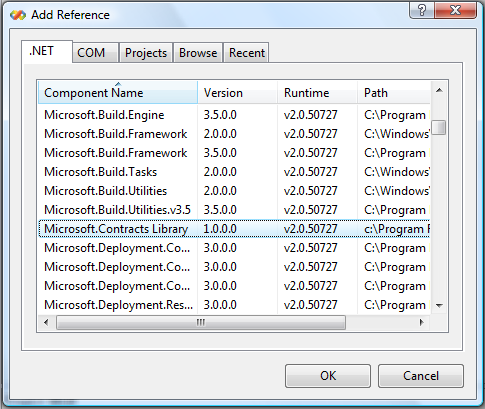
\includegraphics[width=.7\columnwidth]{../Common/addRef.png}
\end{center}



\section{A Simple Protocol: Nullable}
\label{sec:start}

Let's start by running the project with contract checking enabled. Go
to the Properties of both projects \textsf{Client} and \textsf{\ProjectName}, select the Code
Contracts pane (at the bottom), and enable runtime and static checking
by clicking on the appropriate boxes, as shown in this screenshot:
\begin{center}
  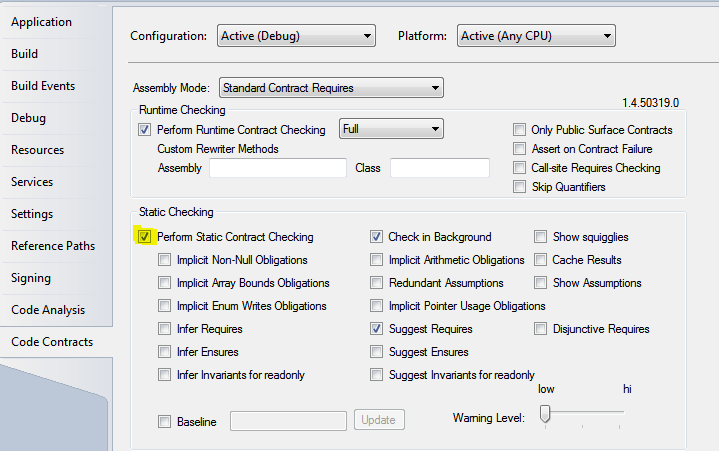
\includegraphics[width=.8\columnwidth]{pane.png}
\end{center}

Then build the solution and run it (or hit F5). You should get an
\textsf{InvalidOperation} exception in method \textsf{Sum} because we
are trying to get the \textsf{Value} of an optional int which has no value.

You are probably familiar with nullable types in C\#. Here, we are
using nullable ints. A nullable int can hold an integer value or no
value. The method \code{Value} on nullables throws an exception if
called on nullables that have no value. Thus this type has a very
simple protocol:
\begin{quote}
To call \code{optX.Value}, \code{optX.HasValue} must be true.
\end{quote}
Stop the execution and look at the warning list (if no warnings
are displayed, rebuild Client).
You should see the static checker warn about the misuse of the
nullable \textsf{optX}:
\begin{center}
  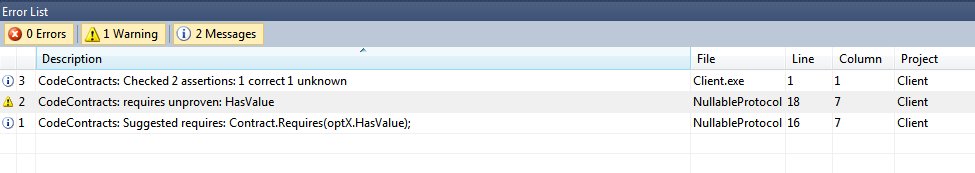
\includegraphics[width=1\columnwidth]{errors1.png}
\end{center}
Double click on the warning stating
that the requires HasValue is unproven. This should take you to the
the spot we just hit in the debugger.

We specified this contract for the Nullable type (we'll show you in a
minute how to specify such contracts). The code here is trying to use
a nullable argument \code{optX} without knowing if
\code{optX.HasValue} is true. The checker complains about this. Note
that the access on the second nullable value \code{optY} is correct,
as it tests for \code{HasValue} first.

Fix the code so it won't bother us in future, e.g., mimicking the test
around the access to \code{optY.Value}.
\begin{lstlisting}
if (optX.HasValue) result += optX.Value;
\end{lstlisting}

\section{A Class with a Protocol}
Now let's take a look at class \code{ClassWithProtocol}. Objects of
this type go through different phases. After construction, an object
of this type must be initialized by calling \code{Initialize} before
any other operation can be meaningfully performed. E.g., property
\code{Data} returns the data passed to \code{Initialize} and thus
should not be called prior to \code{Initialize}. Similarly, property
\code{ComputedData} is only available after additionally calling
\code{Compute}.

Such a protocol can be described by thinking of the object as being in
one of three different states: \code{NotReady, Initialized, Computed}.
The following table shows what operations are available in each state
and how the object's state changes according to the operations:

\begin{tabular}{|l|l|p{2in}|}
\hline
State & Allowed Operations & New state(s)
\\
\hline
\hline
- & Constructor & NotReady
\\
\hline
NotReady & Initialize & Initialized
\\
\hline
Initialized & Data, Compute & unchanged after Data, Computed (after
Compute)
\\
\hline
Computed & Data, ComputedData & unchanged
\\
\hline
\end{tabular}

To save you some typing, we already wrote the contracts for this
protocol. You can find them in the file
\code{ClassWithProtocolFinal}. Feel free to copy-paste from there as
we go through adding contracts in the rest of this sample.

\section{Adding the State}
There are many ways we could make the state of the object
explicit, e.g., through multiple properties. The simplest way is to
use an actual \code{State} property and an enum listing the states as
we had in our table above.

Add the following code in \code{ClassWithProtocol} to keep track of
what state the object is in:
\begin{lstlisting}
  public enum S {
    NotReady, Initialized, Computed
  }

  private S _state;
  public S State
  {
    get
    {
      return _state;
    }
  }
\end{lstlisting}
Now it makes sense to update the state in each operation according to
our table. Thus, in the constructor, we set the state to
\code{NotReady}.
\begin{lstlisting}
  public ClassWithProtocol()
  {
    _state = S.NotReady;
  }
\end{lstlisting}
Similarly, in \code{Initialize} and \code{Compute}, we set the state
to \code{Initialized} and \code{Computed} respectively.
\begin{lstlisting}
  public void Initialize(string data)
  {
    this._data = data;
    _state = S.Initialized;
  }

  public void Compute(string prefix)
  {
    this._computedData = prefix + _data;
    _state = S.Computed;
  }
\end{lstlisting}
Now, so far all we have done is make the state of our object
explicit. That was the most important step, since now we can actually
specify how to use this class. E.g., we can now add pre-conditions to
all method to specify what state(s) the object needs to be in so the
operation makes sense.

Let's first do the two properties. According to our table, the
\code{Data} property is accessible in all states but the
\code{NotReady} state. We can easily specify this by the following
contract:
\begin{lstlisting}
  public string Data
  {
    get
    {
      Contract.Requires(State != S.NotReady);

      return _data;
    }
  }
\end{lstlisting}
An important thing to note here is that we used the publicly visible
property \code{State} and not our private backing field
\code{_state}. It is important that contracts that callers must
observe are visible to callers!

For the \code{ComputedData} property, the state must be equal to
\code{Computed}. So we add the following:
\begin{lstlisting}
  public string ComputedData
  {
    get
    {
      Contract.Requires(State == S.Computed);

      return _computedData;
    }
  }
\end{lstlisting}

Now let's add the appropriate pre-conditions to the two remaining
methods: \code{Initialize} requires \code{NotReady}, and
\code{Compute} requires \code{Initialized}.
\begin{lstlisting}
  public void Initialize(string data)
  {
    Contract.Requires(State == S.NotReady);

    this._data = data;
    _state = S.Initialized;
  }

  public void Compute(string prefix)
  {
    Contract.Requires(State == S.Initialized);

    this._computedData = prefix + _data;
    _state = S.Computed;
  }
\end{lstlisting}

At this point, we have enough contracts for runtime checking the
protocol on clients. Hit F5 to compile and run. The execution should
stop with the following message:
\begin{center}
  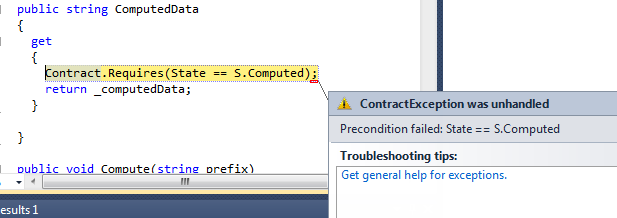
\includegraphics[width=.6\columnwidth]{assertion1.png}
\end{center}
If you look at the call stack, you see that the execution is stopped
at the point where we access the \code{ComputedData} property, but the
state of our object is \code{Initialized}.

\section{Making Static Checking Work}
The specifications in the previous section are enough to catch errors
\emph{at runtime} made by the client. In order to catch errors in the
implementation, we
need contracts that specify how the methods change the state, in
particular, what state is ensured by each method. These
same contracts also allow the static checker to catch these errors at
build time.

Properties are assumed to be pure and thus don't change the state. We
therefore don't need to specify a post state for them. According to
our table, we add the following post-condition to the constructor:
\begin{lstlisting}
    Contract.Ensures(this.State == S.NotReady);
\end{lstlisting}
Similarly, we add the following to \code{Initialize}:
\begin{lstlisting}
    Contract.Ensures(this.State == S.Initialized);
\end{lstlisting}
and the following to \code{Compute}:
\begin{lstlisting}
    Contract.Ensures(this.State == S.Computed);
\end{lstlisting}
These contracts make sure that the implementation actually matches our
table of state transitions. Suppose we forgot to update the
\code{_state} variable in one of our methods. These specifications
will catch that.

If you rebuild the solution now, you should get the following warning
from the static contract checker:
\begin{center}
  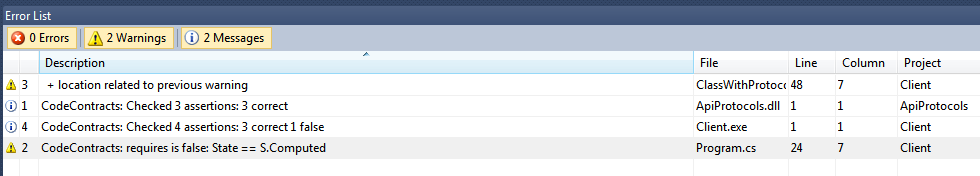
\includegraphics[width=1\columnwidth]{errors2.png}
\end{center}
Double-clicking on the warning takes you to the access of
\code{ComputedData} that failed with the runtime check as expected. We
can now fix the client code by calling \code{Compute} before accessing
\code{ComputedData}.
\begin{lstlisting}
      c.Compute("whatever");
      var data = c.ComputedData;
\end{lstlisting}
Now running the code produces no runtime error, and the static checker
will produce the following output:
\begin{center}
  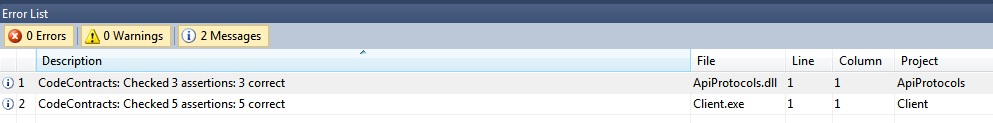
\includegraphics[width=1\columnwidth]{errors3.png}
\end{center}

\section{Taking Advantage of State Invariants}
Now that we have our protocol setup, we can strengthen the post
conditions on our properties. It would be nice to guarantee that the
properties always return non-null strings. Let's start by turning on
non-null checking by selecting the \code{Properties} on each project
by selecting the implicit non-null checkbox.

Building should produce a warning that \code{data} (the result of
\code{ComputedData}) might be null in the \code{Main} method.
Let's look at the \code{ClassWithProtocol} code again. If we require
the argument to \code{Compute} to be non-null, then clearly, if we
are in the \code{Computed} state, the field \code{_computedData}
should be non-null. We add the following contracts to make this
explicit. On \code{Compute}, let's add the following requires (recall
that you can use the \code{crn TAB TAB} snippet):
\begin{lstlisting}
    Contract.Requires(prefix != null);
\end{lstlisting}
We also add the following ensures on the \code{ComputedData} getter
(the \code{cen TAB TAB} snippet will do it):
\begin{lstlisting}
      Contract.Ensures(Contract.Result<string>() != null);
\end{lstlisting}
If you build now, you should get the following output:
\begin{center}
  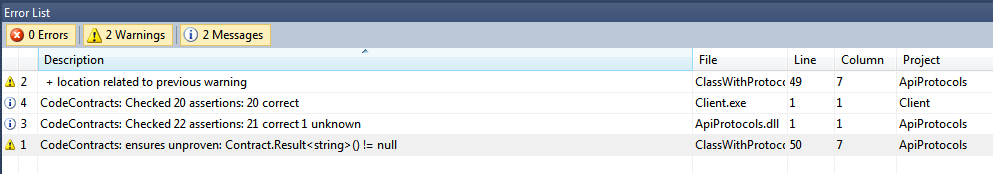
\includegraphics[width=1\columnwidth]{errors4.png}
\end{center}
The checker is now happy with the client code and can guarantee that
the \code{ComputedData} value is non-null. However, it cannot yet
prove the ensures of that getter in the implementation. The reason is
that the invariant relating the \code{_state} and the non-nullness of
\code{_computedData} is not evident to the checker. We can help it by
specifying the following object invariant in \code{ClassWithProtocol}.
\begin{lstlisting}
  [ContractInvariantMethod]
  protected void ObjectInvariant()
  {
    Contract.Invariant(_state != S.Computed || _computedData != null);
  }
\end{lstlisting}
The invariant specifies that either we are not in the \code{Computed}
state, or field \code{_computedData} is non-null. Building now should
return no more warnings, as the checker can make sure that every
method actually satisfies this invariant.

As an exercise, you can try adding a similar invariant that specifies
that \code{_data} is non-null in all states but the \code{NotReady}
state.

\section{Conditional Transitions}
Not all protocols are as straight-forward as the one we have seen so
far. Often, methods may have multiple outcomes. For example, suppose
\code{Compute} had to access the file system and could only compute
the proper value if a particular file was there. Thus, the method
would not transition the state to \code{Computed} in all cases.

To examine this possibility,  let's modify \code{Compute} so it
returns a \code{bool} to indicate whether it succeeded in the
computation. Otherwise, the state of the object remains
\code{Initialized}, so the computation could be attempted again.
To specify this, we modify the existing ensures contract to the
following one:
\begin{lstlisting}
  public bool Compute(string prefix)
  {
    Contract.Requires(prefix != null);
    Contract.Requires(State == S.Initialized);
    Contract.Ensures(Contract.Result<bool>() && State == S.Computed ||
                     !Contract.Result<bool>() && State == S.Initialized);
\end{lstlisting}
Don't forget to also return a boolean value. Since we haven't
implemented the failing case, let's just return true. Building now
should produce a warning in the client code that \code{State ==
  S.Computed} might be false at the call to the \code{ComputedData}
getter. In order for the client to satisfy the protocol, it must check
the return value of \code{Compute}.

If we modify the client as follows:
\begin{lstlisting}
      if (c.Compute("whatever"))
      {
        var data = c.ComputedData;

        Console.WriteLine(data.ToString());
      }
\end{lstlisting}
the warning disappears. We have thus successfully refined the protocol
of our class and automatically found client code that needed to be
adjusted to our change.

\end{document}
